\chapter{Принцип измерения ЭДМ методом ``замороженного спина'' (FS)}\label{chpt1:top-level}

\section{Общее введение в методологию}\label{chpt1:FS-introduction}

\subsection{Уравнение Т-БМТ}\label{sec:TBMT_introduction}
Уравнение Томаса-Баргманна-Мишеля-Телегди описывает динамику спин-вектора $\vec s$ в
магнитном поле $\vec B$ и электростатическом поле $\vec E$. Его
обобщённая версия, включающая влияние ЭДМ, может быть записана (в
системе центра масс пучка) как:~\cite[стр.~6]{Eremey:Thesis}
\begin{subequations}
	\begin{align}
		\ddt{\vec s} &= \vec s\times \bkt{\vec\W_{MDM} +\vec\W_{EDM}}, \label{eq:TBMT_main}
		\intertext{где МДМ и ЭДМ угловые скорости $\vec\W_{MDM}$ и $\vec\W_{EDM}$ }
		\vec\W_{MDM} &= \frac{q}{m\gamma} \bkt*{(\gamma G + 1)\vec B - \bkt{\gamma G + \frac{\gamma}{\gamma+1}}\frac{\vec\beta\times\vec E}{c}},\label{eq:TBMT_MDM} \\
		\vec\W_{EDM} &= \frac qm \frac\eta2 \bkt*{\vec\beta\times \vec B + \frac{\vec E}c}.\label{eq:TBMT_EDM}
	\end{align}
\end{subequations}
В уравнениях выше, $m,~q,~G=(g-2)/2$ есть, соответственно, масса, заряд, и
магнитная аномалия частицы; $\beta = \sfrac{v_0}{c}$,
нормализованная скорость частицы; $\gamma$ её Лоренц-фактор. ЭДМ
множитель $\eta$ определяется уравнением $d = \eta\frac{q}{2mc}s$, где
$d$ --- ЭДМ частицы, а $s$ её спин.

В стандартном формализме принято оперировать с матрицей преобразования (поворота) спина за оборот в кольце $R$:~\cite[стр.~4]{COSY:SpinTuneMapping}
\[
\bold{t}_R = \exp\bkt{-i\pi\nu_s\vec\sigma\cdot\bar n} = \cos\pi\nu_s - i (\vec\sigma\cdot\bar n)\sin\pi\nu_s,
\]

где $\nu_s = \sfrac{\W_s}{\W_{cyc}}$ отношение угловой скорости поворота спин-вектора частицы к её циклотронной частоте, называемое \emph{спин-тюн}, а $\bar n$ определяет направление оси прецессии спина, и называется \emph{инвариантной спиновой осью}.

\subsection{Концепция замороженного спина}
Из уравнения~\eqref{eq:TBMT_MDM} можно видеть, что, в отсутствии ЭДМ,
направление вектора спина частицы пучка может быть зафиксировано
относительно её вектора импульса: $\vec\W_{MDM}=\vec 0$; иными словами, можно реализовать
условие замороженности спина (Frozen Spin condition).

Достоинство работы в FS-состоянии в накопительном кольце
следующее: в соответствии с
уравнениями~\cref{eq:TBMT_main,eq:TBMT_MDM,eq:TBMT_EDM}, векторы МДМ и
ЭДМ угловых скоростей ортогональны, а потому в общей скорости
прецессии они складываются квадратично, в связи с чем сдвиг частоты
прецессии, связанный с ЭДМ, становится эффектом второго порядка
величины:~\cite[стр.~5]{Mane:SpinWheel}
\[
\w \propto \sqrt{\W_{MDM}^2 + \W_{EDM}^2} \approx \W_{MDM} + \frac{\W_{EDM}^2}{2\W_{MDM}}.
\]
Это обстоятельство значительно ухудшает чувствительность эксперимента.

Однако, заморозив спин в горизонтальной плоскости, единственная
остающаяся МДМ компонента угловой скорости сонаправлена с ЭДМ
компонентой, а значит складывается с ней линейно. Таким образом,
чувствительность значительно улучшается.

\subsection{Реализация условия замороженности спина в накопительном кольце}\label{sec:FS_in_a_ring}
Накопительные кольца могут быть классифицированы в три группы:
\begin{enumerate}
	\item чисто магнитные (как COSY, NICA, etc),
	\item чисто электростатические (Brookhaven AGS Analog Ring),
	\item комбинированные.
\end{enumerate}

Ввиду уравнения~\eqref{eq:TBMT_MDM}, условие FS не может быть
выполнено в чисто магнитном кольце.

Для некоторого числа частиц, таких как протон, чья $G>0$, чисто
электростатическое кольцо может быть использовано в рамках FS
методологии ЭДМ эксперимента с пучком на так называемой ``магической''
энергии, определяемой как $\gamma_{mag} = \sqrt{(1+G)/G}$.

Для частиц с $G<0$ (таких как дейтрон),это невозможно, и необходимо
использовать комбинированное кольцо. Для того, чтобы реализовать FS
условие в комбинированном кольце, вводится ~\cite{BNL:Deuteron2008} радиальное электрическое
поле величины
\begin{equation}\label{eq:FS_Er}
E_r = \frac{GB_yc\beta\gamma^2}{1-G\beta^2\gamma^2}.
\end{equation}

\section{Методы, основанные на FS методологии}\label{chpt1:FS-methods}
В этом разделе мы сначала приведём два основополагающих примера методов поиска ЭДМ
в накопительном кольце, основанных на принципе замороженного спина;
затем обобщим  эти методы до двух взаимоисключающих категорий;
и завершим описанием метода Frequency Domain.

Отметим, что помимо метода замороженного спина существуют альтернативные подходы к измерению ЭДМ, например~\cite{COSY:SpinTuneMapping, COSY:Partially-Frozen-Spin}, в котором поляризация пучка свободно вращается вокруг вертикального ведущего поля ускорителя.

\newcommand{\wimp}{\w_{\avg{E_v}}}
\newcommand{\wsw}{\w_{SW}}
\newcommand{\wedm}{\w_{edm}}

\newcommand{\D}{\Delta}
\DeclareDocumentCommand{\g}{s}{\gamma\IfBooleanT{#1}{_{eff}}}

\subsection{Метод BNL FS}
BNL FS метод, предложенный коллаборацией, занимающейся разработкой
метода измерения ЭДМ в накопительном кольце в Брукхейвенской
Национальной Лаборатории (США) в 2008 году,~\cite{BNL:Deuteron2008}
это метод для комбинированного кольца. Пучок продольно-поляризованных
дейтронов инжектируется в кольцо; с помощью поляриметрии наблюдается
его спин-прецессия в вертикальной и горизонтальной плоскостях; ЭДМ
сигнал --- это изменение вертикальной компоненты поляризации со
временем, выражаемое как:~\cite[стр.~8]{BNL:Deuteron2008}
\begin{equation}
  \Delta P_V = P\frac{\w_{edm}}{\W}\sin\bkt{\W t + \Theta_0},
\end{equation}
где $\W = \sqrt{\w_{edm}^2 + \w_a^2}$, $\w_a,~\w_{edm}$ угловые
скорости вызываемые, соответственно, магнитным и электрическим
дипольными моментами.

Прилагая радиальное магнитное поле $E_r$ (величины, определяемой уравнением~\eqref{eq:FS_Er}), ожидается
уменьшение компоненты $\w_a$ по крайней мере на фактор $10^9$; ввиду
малости величины гипотезируемой $\w_{edm}$, $\Delta P_V \approx P
\w_{edm} t$, и максимальная величина $\Delta P_V$ возрастает в $10^9$.

Ожидаемая чувствительность эксперимента $10^{-29}~e\cdot cm$ за $10^7$
секунд (6 месяцев) полного времени измерения. На этом уровне
чувствительности, асимметрия сечения $\varepsilon_{LR} \approx 5\cdot
10^{-6}$ для наименьших практически реализуемых значений
$\w_a$.~\cite[стр.~18]{BNL:Deuteron2008} Последнее обстоятельство
ставит серьёзную проблему для поляриметрии.~\cite{Mane:SpinWheel} Один
из вариантов её решения лежит в применении внешнего радиального
магнитного поля и измерении общей частоты прецессии засчёт МДМ и ЭДМ
вместе. Это основа так называемого метода Спинового Колеса (Spin Wheel), также 
часто называемого Кооп-Колесом (Koop Wheel), о котором в
следующем разделе. 

Единственный известный систематический эффект спиновой динамики
первого порядка это присутствие ненулевой средней вертикальной
компоненты электрического поля $\avg{E_V}$. В этом случае, спин будет
прецессировать вокруг радиального направления с частотой~\cite[стр.~11]{BNL:Deuteron2008}
\[
\w_{syst} \approx \frac{\mu\avg{E_V}}{\beta c\gamma^2}.
\]
Здесь важно рассмотреть два обстоятельства:
\begin{itemize}
\item присутствие $\avg{E_V}\neq 0$ вызвано ошибкой юстировки
  элементов ускорителя;
\item этот систематический эффект меняет знак при инжекции пучка в
  обратном направлении.
\end{itemize}
Последнее обстоятельство является причиной структуры инжекции пучка
использованной в этом методе (сначала по-часовой, потом
против-часовой; CW/CCW). Хотя $\w_{syst}$ меняет знак при смене
направления движения пучка а значит поддаётся контролю, эта методология тем не менее не учитывает
его \emph{величину}. В разделе~\ref{chpt3:imperfections} (численно в~\ref{chpt3:imperfections:magnitude}), 
мы показываем, что при реалистичной величине (стандартного отклонения) ошибки установки
спин-ротаторов 100 мкм, частота МДМ прецессии вокруг радиальной оси
находится на уровне 50--100 рад/сек.~\cite{Senichev:FDM} В связи с
этим, невозможно использовать данную методологию в её оригинальном варианте.

Также, стоит отметить, что при попытке уменьшения $\w_{syst}$, увеличивается влияние
так называемой ошибки геометрической фазы.~\cite[стр.~6]{BNL:Proton}

\subsection{Spin Wheel метод}
Озвученные выше проблемы с поляриметрией и высокой скоростью прецессии
решаются в Spin Wheel методе, предложенном проф. И. Коопом
(Новосибирский Государственный Университет).~\cite{Koop:SpinWheel} Основная идея метода в
следующем: сначала, обеспечивается условие замороженного спина; затем
включается радиальное магнитное поле величины $B_x$, достаточно сильное чтобы
вызвать вращение спина с частотой порядка 1 Гц. Поскольку поле
радиальное, вызванная им МДМ прецессия сонаправлена с ЭДМ, а значит
они складываются линейно: $\w \propto \W_{MDM} + \W_{EDM}$.

ЭДМ вклад вычисляется сравнением циклов с противоположными знаками $B_x$:~\cite[стр.~1963]{Koop:SpinWheel}
\[
\W_{EDM} = \frac{\W_x(+B_x) + \W_x(-B_x)}{2}.
\]

Внешнее поле также вызовет разделение орбит
пучков.~\cite[стр.~1963]{Koop:SpinWheel} Это разделение может быть
измерено на уровне пико-метров SQUID магнетометрами; его предлагается
использовать для калибровки внешнего поля.

Поскольку из-за внешнего поля прецессия вокруг радиальной оси на 10
порядков выше чем в оригинальном предложении, значительно упрощается
задача для поляриметрии. Однако, существуют сомнения в возможности
измерить вызываемое внешним полем разделение орбит даже при помощи SQUIDов.

Также, проблема паразитного поля, вызванного ошибкой юстировки, не решена.

\subsection{Общая классификация методов FS-типа}
Методы поиска электрического дипольного момента элементарных частиц можно отнести к одной из 
двух больших категорий, которые мы будем называть 
\begin{enumerate*}[\itshape a\upshape)]
	\item методами пространственной области (Space Domain methods), и
	\item методами частотной области (Frequency Domain methods).
\end{enumerate*}

В парадигме пространственной области, наблюдают за \emph{изменением пространственной
ориентации} вектора поляризации пучка, \emph{вызванным ЭДМ}. 

Метод BNL FS --- это канонический пример методологии пространственной области: изначально
продольно-поляризованный пучок инжектируется в накопительное кольцо; наблюдают за 
вертикальной компонентой его вектора поляризации. При идеальных условиях, любое отклонение
вектора поляризации от горизонтальной плоскости связывают с действием ЭДМ.

Сразу же очевидны две технические проблемы такого подхода:
\begin{enumerate}
	\item он ставит трудную задачу для поляриметрии~\cite{Mane:SpinWheel};
	\item он налагает очень строгие ограничения на точность установки оптических элементов ускорителя.
\end{enumerate}

Первая проблема обусловлена необходимостью детектирования изменения асимметрии сечения 
взаимодействия $\epsilon_{LR}$ на уровне $5\cdot 10^{-6}$, чтобы достичь уровня чувствительности
ЭДМ $10^{-29}~e\cdot$см.~\cite[стр.~18]{BNL:Deuteron2008}

Вторая --- требованием минимизировать величину угловой скорости МДМ прецессии в 
вертикальной плоскости~\cite[стр.~11]{BNL:Deuteron2008}
\begin{equation}\label{eq:ImperfectionWheelRollRate}
	\w_{syst} \approx \frac{\mu\avg{E_v}}{\beta c\gamma^2},
\end{equation}
индуцированной неидеальностями ускорителя. 

В соответствии с оценками, сделанными проф. Сеничевым, чтобы выполнить это условие,
геодезическая точность установки элементов ускорителя должна достичь $10^{-14}$ м. 
Технологии сегодняшнего дня позволяют получить только около $10^{-4}$ м.

При практически-достижимом уровне неточности установки элементов, $\w_{syst}\gg\w_{edm}$,
и изменения ориентации вектора поляризации по большей части не имеют отношения к ЭДМ.

Другой критичной проблемой, возникающей в пространственной области, является ошибка
геометрической фазы.~\cite[стр.~6]{BNL:Proton}  Проблема заключается в том, что даже если
каким-то образом занулить неидеальности электромагнитного поля (связанные с неточностью
установки оптических элементов, или же случайными возмущениями поля) \emph{в среднем},
поскольку повороты спина не коммутируют, угол поворота поляризации, вызванный ими, не 
будет равен нулю.

Напротив, методология частотной области основана на измерении ЭДМ-\emph{добавки} к полной
(МДМ и ЭДМ вместе) \emph{угловой скорости} прецессии спина.

Вектор поляризации заставляют вращаться вокруг почти-постоянного, выделенного направления,
определённого вектором $\nbar$, с достаточно высокой угловой скоростью, при которой её
величину можно всегда легко измерить. Помимо упрощения условий поляриметрии, определённость
вектора угловой скорости является защитой от ошибки геометрической фазы.

Так называемое Спин-Колесо может быть введено в систему извне, как в методе Spin Wheel; или же
под ту же цель можно приспособить поля неидеальности машины (скорость вращения колеса 
определяется уравнением~\eqref{eq:ImperfectionWheelRollRate}). Последнее возможно потому,
что $\w_{syst}$ меняет знак при смене направления движения пучка.~\cite[стр.~11]{BNL:Deuteron2008}

\subsection{Общие проблемы методов поиска ЭДМ в накопительном кольце}\label{sec:FSSREDM:problems}
В качестве введения в предлагаемую методологию частотной области, коротко суммаризируем 
некоторые проблемы, общие для всех методов поиска ЭДМ в накопительном кольце; их можно
разделить на две большие категории:

\begin{itemize}
	\item Проблемы, решаемые Спин-Колесом:
	\begin{itemize}
		\item случайные возмущения электромагнитного поля;
		\item бетатронное движение.
	\end{itemize}
	\item Проблемы, имеющие частные решения:
	\begin{itemize}
		\item декогеренция спина;
		\item неидеальности ускорителя.
	\end{itemize}
\end{itemize}

\subsubsection{Возмущения спиновой динамики}
Проблемы первой категории --- это такие, из-за которых возникает ошибка геометрической фазы.

И случайно-возникающие, и фокусирующие поля, действуя на бетатронно-осциллирующую частицу,
возмущают направление и величину вектора угловой скорости спин-прецессии. Эффектом является
спин-кик в направлении, определяемом возмущением.

Положим ЭДМ создаёт спин-кик вокруг радиальной ($\hat x$-) оси. Величина вектора угловой скорости
имеет общую форму
\[
\w = \sqrt{\w_x^2 + \w_y^2 + \w_z^2},
\]
где  $\w_y$ минимизируется путём удовлетворения условия замороженного спина; $\w_z$ (чья постоянная
составляющая вызвана неидеальностями ускорителя) может быть минимизирована установкой продольного 
соленоида на оптической оси.\footnote{Длины 1 м, магнитное поле приблизительно $10^{-6}$ Т.}

В пространственной области, стремятся также минимизировать добавку $\wimp$ к радиальной компоненте
угловой скорости $\w_x = \w_{edm} + \wimp$. Следовательно, и спин-кики должны быть минимизированы до
величины (значительно) меньшей чем $\w_{edm}$, чтобы понизить набег геометрической фазы до значений
меньших, чем аккумулированная ЭДМ фаза.

Польза от Спин-Колеса, сонаправленного с угловой скоростью угловой скорости ЭДМ состоит в том, что
МДМ добавки к общей угловой скорости складываются как квадраты, а потому, их эффект значительно уменьшен:
\begin{align*}
	\w &= \sqrt{(\wedm + \wsw)^2 + \w_y^2 + \w_z^2} \\
	&\approx (\wedm+\wsw)\cdot\bkt*{1 + \frac{\w_y^2 + \w_z^2}{\wsw^2}}^{\sfrac12} \\
	&\approx (\wedm + \wsw)\cdot \bkt{1 + \frac{\w_y^2 + \w_z^2}{2\wsw^2}} \\
	&\approx \wsw + \wedm + \underbrace{\frac12\frac{\w_y^2 + \w_z^2}{\wsw}}_{\epsilon}.
\end{align*}

Поскольку наша цель --- наблюдение смещения значения $\w$, связанное с ЭДМ, необходимо 
минимизировать случайную переменную $\epsilon$:
\[
\frac12\frac{\w_y^2+\w_z^2}{\wsw} < \wedm.
\]

Сделаем предварительные оценки. Положим $\wsw\approx 50$ рад/сек (причины выбора этого значения
разъяснены в разделе~\ref{chpt3:imperfections}), $\wedm\approx 10^{-9}$ рад/сек (соответствует величине
ЭДМ $10^{-29}~e\cdot$см). Тогда, сумма $\w_y^2 + \w_z^2$ должна быть меньше $10^{-7}$ рад/сек, или
же каждая из угловых скоростей меньше $3\cdot 10^{-4}$ рад/сек. Это на несколько порядков меньше,
чем ожидаемая стандартная ошибка оценки угловой скорости,~\cite{Aksentev:Stats} и потому не является проблемой.

Остаётся рассмотреть МДМ спин-кики вокруг $\hat x$-оси; они не аттеньюированы, вызывают наибольшие проблемы.
Их можно поделить на три вида: 
\begin{enumerate*}[\itshape a\upshape)]
	\item постоянные, не индуцированные ошибкой юстировки оптических элементов;
	\item полу-постоянные, индуцированные ошибками юстиорвки;
	\item случайные.
\end{enumerate*}

Полу-постоянные радиальные спин-кики (не важно, вызванные ли магнитными, или электрическими полями) меняют
знак, когда обращается направление циркуляции пучка. Влияние случайных спин-киков можно контролировать 
статистическим усреднением. Перманентные, нечувствительные ни к направлению ведущего поля, ни к направлению
движения пучка, не поддаются контролю. Но с другой стороны, их источники не должны присутствовать в ускорителе
при нормальных обстоятельствах. Мы рассматриваем влияние возмущений спиновой динамики пучка на измерение
ЭДМ в разделе~\ref{chpt3:smp}.

\subsubsection{Декогеренция спина}
Когеренцией спина называется мера или качество сохранения поляризации
в изначально полностью поляризованном пучке.~\cite[стр.~205]{Eremey:Thesis}
Под декогеренцией спина понимают деполяризацию, связанную с различием угловых скоростей 
частиц пучка. 

Разница угловых скоростей, в свою очередь, связана с разницей длин орбит частиц, и следовательно
их уровней равновесной энергии, от которых зависит спин-тюн. Одним из способов подавления декогеренции
спина является утилизация секступольных полей. Как это работает, мы рассматриваем в рвзделе~\ref{chpt3:decoherence}.

\subsubsection{Неидеальности ускорителя}
Как мы уже указывали, проблема неидеальностей ускорителя имеет две стороны:
\begin{enumerate*}[\itshape a\upshape)]
	\item они практически не могут быть убраны настоящини технологиями; но что ещё хуже
	\item если их убрать, мы попадаем в пространственную область, и открываем метод для геометрической фазы.
\end{enumerate*}

К счастью, спин-кики, возбуждаемые ими, меняют знак при смене направления движения пучка. К тому же,
их величина достаточна, чтобы использовать их в качестве Спин-Колеса. Подробнее, вопрос МДМ прецессии, связанной с полями неидеальности ускорителя, рассматривается в разделе~\ref{chpt3:imperfections}.

Остаётся одна проблема: точность установки скорости вращения колеса при смене его направления. Этот момент
рассматривается в разделе~\ref{chpt3:GFF}.

\subsection{Метод Frequency Domain}\label{sec:FDM_concept}
\subsubsection{Главные особенности}
Предлагаемый метод обладает следующими основными характеристиками:
\begin{enumerate}
	\item Это метод временной области;
	\item Вместо подавления, поля, связанные с неидеальностями ускорителя, используются в качестве Спин-Колеса.
	\begin{itemize}
		\item Смена направления вращения Спин-Колеса производится сменой полярности ведущего поля ускорителя;
		\item контроль скорости его вращения производится на основе наблюдения прецессии спина в горизонтальной плоскости.
	\end{itemize}
\end{enumerate}

Мы уже рассмотрели достоинства частотной области, такие как 
\begin{enumerate}[\itshape a\upshape)]
	\item упрощение поляриметрии, и 
	\item иммунитет к ошибке геометрической фазы.
\end{enumerate}
Уделим более пристальное внимание вопросу использования полей неидеальности ускорителя в качестве Спин-Колеса.

\subsubsection{ЭДМ-статистика}
Поскольку угловая скорость измеряемая в методологии частотной области включает добавки и от
магнитного, и от электрического, дипольных моментов, для построения ЭДМ-эстиматора требуется использование двух циклов:
в первом МДМ вращение происходит в одну сторону, во втором в обратную.

В связи с тем, что Кооп-Колесо в FDM --- это продукт ведущего поля, для обращения направления его вращения 
необходимо поменять полярность ведущего поля.
Когда это происходит:
$\vec B \mapsto -\vec B$, направление циркуляции пучка изменяется с по-часовой (CW) до против-часовой (CCW): 
$\vec\beta \mapsto -\vec\beta$, в то время как электростатическое поле остаётся неизменным: $\vec E \mapsto \vec E$.
В соответствии с уравнением Т-БМТ, компоненты частоты прецессии спина меняются как:
\begin{subequations}
	\begin{align}
	\w_x^{CW} &= \w_x^{MDM, CW}   + \w_x^{EDM}, \notag\\
	\w_x^{CCW} &= \w_x^{MDM, CCW} + \w_x^{EDM}, \notag\\
	\w_x^{MDM, CW} &= -\w_x^{MDM, CCW}, \label{eq:CW_CCW_MDM}\\
	\intertext{и ЭДМ-эстиматор}
	\hat\w_x^{EDM} &:= \frac12\bkt{\w_x^{CW} + \w_x^{CCW}} \label{eq:FDM_estimator} \\
	&=  \w_x^{EDM} +
	\underbrace{\frac12\bkt{\w_x^{MDM, CW} + \w_x^{MDM, CCW}}}_{\varepsilon \to 0}.
	\end{align}
\end{subequations}

Для того, чтобы удерживать систематическую ошибку $\varepsilon$ ниже уровня требуемой точности, т.е. гарантировать что условие~\eqref{eq:CW_CCW_MDM} выполняется с достаточной точностью, проф. Сеничев 
разработал~\cite{Senichev:FDM} процедуру смены полярности ведущего поля,
основанную на наблюдении частоты прецессии поляризации пучка в горизонтальной плоскости. 
Принцип работы процедуры описан в разделе~\ref{chpt3:GFF}; для его объяснения необходимо ввести понятие эффективного Лоренц-фактора (см. раздел~\ref{chpt1:FS-methods:effective-Lorentz-factor}).

\subsubsection{Метод оценки частоты и  свойства данных}
Подробно вопрос оценки частоты рассмотрен в приложении~\ref{Apx:Stats}. В настоящем разделе, вкратце опишем лишь основные заключения.

Во-первых, частота прецессии поляризации пучка оценивается путём фитирования данных поляриметрии синусоидальной функцией с постоянными параметрами. В связи с этим, возникает проблема возмущения спиновой динамики (например, связанное с бетатронными колебаниями), рассматриваемая в разделе~\ref{chpt3:smp}. По результатам проведённого анализа, мы заключаем что этот эффект не составляет проблему в рамках предлагаемой методологии.

Во-вторых, данные поляриметрии обладают свойством \emph{гетероскедастичности},  т.е. ошибка измерения поляризации пучка растёт к концу измерительного цикла.~\cite{Eversmann:Thesis} Обыкновенный метод наименьших квадратов (Ordinary Least Squares) теряет эффективность при фитировании данных, обладающих таким свойством; также, даваемые им стандартные ошибки оценок параметров оказываются смещены и несостоятельны. При этом, ожидания оценок остаются валидными. Поэтому, при использовании OLS необзодимо использовать стандартные ошибки в форме Уайта. Но лучше вместо OLS использовать гетероскедастичные модели.~\cite{Stats:R:NLREG, Stats:HeteroskedasticNRM}

В-третьих, деполяризация пучка налагает более жёсткие ограничения на длительность измерительного цикла, чем время жизни пучка. Предположим пучок с бесконечным временем жизни.~\footnote{Помимо прочего, это означает недеструктивную поляриметрию.} Очевидно, что когда пучок полностью деполяризуется, мы не сможем получать информацию о скорости вращения его поляризации; т.е. существует принципиальное ограничение на полное количество информации (обозначим её $\mathrm{FI_{tot}}$) о частоте прецессии спина, которое можно получить из одной инжекции. Будем называть период времени, за который поляризация уменьшается в $e$ раз, постоянной времени деполяризации $\tau_d$. В таблице~\ref{tbl:FItot} отражено количество выбранной (относительно $\mathrm{FI_{tot}}$) информации о частоте прецессии спина как функция длительности цикла, а также соответствующее отношение сигнал/шум.~\footnote{Отношение вычислено исходя из модели сигнала поляризации и модели ошибки измерения поляризации.} Исходя из данных таблицы, полезная длительность измерительного цикла ограничена тремя постоянными времени деполяризации.

В четвёртых, наши симуляции показывают возможность достичь точности оценки частоты прецессии спина на уровне $8\cdot 10^{-7}$ рад/сек за один измерительный цикл, при постоянной времени деполяризации 1,000 секунд, частоте измерения поляризации 375 Гц, и начальной ошибке измерения поляризации 3\%. При 70\%  временной загрузке ускорителя, это позволяет выйти на уровень $5\cdot 10^{-9}$ рад/сек стандартного отклонения среднего значения оценки частоты. Такая точность достаточна для получения оценки ЭДМ на уровне $10^{-29}~e\cdot$см.

\begin{table}[h]
	\caption{Количество выбранной информации (в долях от потенциального максимума), в зависимости от длительности измерительного цикла, и соответствующее отношение сигнал/шум.\label{tbl:FItot}}
	
	\centering
	\begin{tabular}{rrr}
		\toprule
		Инфо. (\%$\mathrm{FI_{tot}}$) & Длительность ($\times\tau_d$) & Сигнал/шум  \\
		\midrule
		95            & 3.0                     & 0.4         \\
		90            & 2.3                     & 1.1         \\
		70            & 1.2                     & 5.5         \\
		50            & 0.7                     & 11.7        \\
		\bottomrule
	\end{tabular}
\end{table}


\subsection{Понятие эффективного Лоренц-фактора}\label{chpt1:FS-methods:effective-Lorentz-factor}
Спиновая динамика описывается понятиями \emph{спин-тюна} $\nu_s$ и \emph{оси стабильного спина} $\nbar$.
Спин-тюн зависит от равновесного уровня энергии частицы, выражаемого Лоренц-фактором:
\begin{equation}\label{eq:spin_tune_vs_gamma}
\begin{cases}
\nu_s^B &= \gamma G, \\
\nu_s^E &= \beta^2\gamma\bkt{\frac{1}{\gamma^2-1} - G} \\
&= \frac{G+1}{\gamma} - G\gamma.
\end{cases}
\end{equation}

К сожалению, не все частицы пучка обладают одним и тем же Лоренц-фактором. Частица вовлечённая в 
бетатронное движение имеет более длинную орбиту, и как прямое следствие принципа автофазировки,
в ускорительной структуре использующей ВЧ-резонатор, её равновесный уровень энергии 
должен вырасти. Иначе она не сможет оставаться у пучке. В этом разделе мы анализируем как Лоренц-фактор частицы
должен измениться при учёте бетатронного движения, а также нелинейностей коэффициента сжатия орбиты.

Продольная динамика частицы на референсной орбите накопительного кольца описывается
системой уравнений:
\begin{equation}
\begin{cases}
\ddt{}\D\varphi &= -\w_{RF}\eta\delta, \\
\ddt{}\delta &= \frac{q V_{RF}\w_{RF}}{2\pi h\beta^2E}\bkt{\sin\varphi - \sin\varphi_0}.
\end{cases}
\end{equation}
В уравнениях выше, $\D\varphi = \varphi - \varphi_0$ и
$\delta = \bkt{p-p_0}/{p_0}$ отклонения фазы и нормализованного импульса частицы
от фазы и импульса референсной частицы;
 $V_{RF}$, $\w_{RF}$, соответственно,
 напряжение и частота ВЧ-поля; $\eta = \alpha_0 - \gamma^{-2}$ слип-фактор,
 где $\alpha_0$ есть коэффициент сжатия орбиты, определяемый как $\sfrac{\Delta L}{L} = \alpha_0\delta$,
 $L$ длина орбиты; $h$ гармонической число; $E$ полная энергия частицы.

Решения этой системы формируют семейство эллипсов в плоскости $(\varphi, \delta)$, с общим центром в
точке $(\varphi_0,\delta_0)$ (см. Рисунок~\ref{fig:PSP:Linear}). Однако, если рассматривать частицу вовлечённую в бетатронный колебания, и
учитывать разложение ряда Тэйлора коэффициента сжатия орбиты более высокого порядка
$\alpha = \alpha_0 + \alpha_1\delta$, то первое уравнение системы
трансформируется в:~\cite[p.~2579]{Senichev:IPAC13}
\begin{align*}
\ddt{\D\varphi} = -\w_{RF} \Bigg[\bkt{\frac{\Delta L}{L}}_\beta &+ \bkt{\alpha_0 + \gamma^{-2}}\delta \Bigg.\\
&+ \Bigg.\bkt{\alpha_1 - \alpha_0\gamma^{-2} + \gamma^{-4}}\delta^2\Bigg],
\end{align*}
где $\bkt{\frac{\Delta L}{L}}_\beta = \frac{\pi}{2L}\bkt*{\varepsilon_xQ_x + \varepsilon_yQ_y}$, это
удлинение орбиты, связанное с бетатронным движением; $\varepsilon_x$ и $\varepsilon_y$ 
горизонтальный и вертикальный эмиттансы пучка, и $Q_x$, $Q_y$ горизонтальный и вертикальный тюны.

Решения трансформированной системы более не центрированы на одной точке (см. Рисунок~\ref{fig:PSP:3rd-order}). Удлинение орбиты
и отклонение импульса вызывают сдвиг равновесного уровня энергии:~\cite[p.~2581]{Senichev:IPAC13}
\begin{equation}\label{eq:EquLevMom_shift}
\Delta\delta_{eq} = \frac{\gamma_0^2}{\gamma_0^2\alpha_0 - 1}\bkt*{\frac{\delta_m^2}{2}\bkt{\alpha_1 - \alpha_0\gamma_0{-2} + \gamma_0^{-4}} + \bkt{\frac{\Delta L}{L}}_\beta},
\end{equation}
где $\delta_m$ есть амплитуда синхротронных колебаний.

\begin{figure}[h]\centering
	\subbottom[Линейная теория.\label{fig:PSP:Linear}]{%
	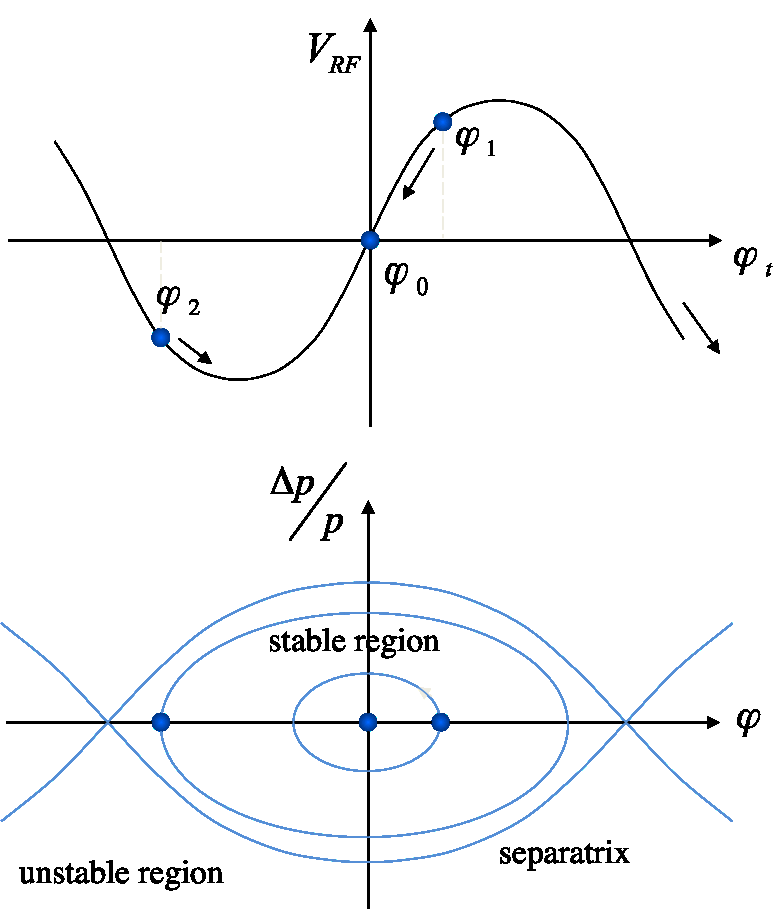
\includegraphics[height=.35\paperheight]{images/chapter1/psp_diagram}}
	\subbottom[Результаты моделирования с трансфер-матрицами третьего порядка.\label{fig:PSP:3rd-order}]{%
	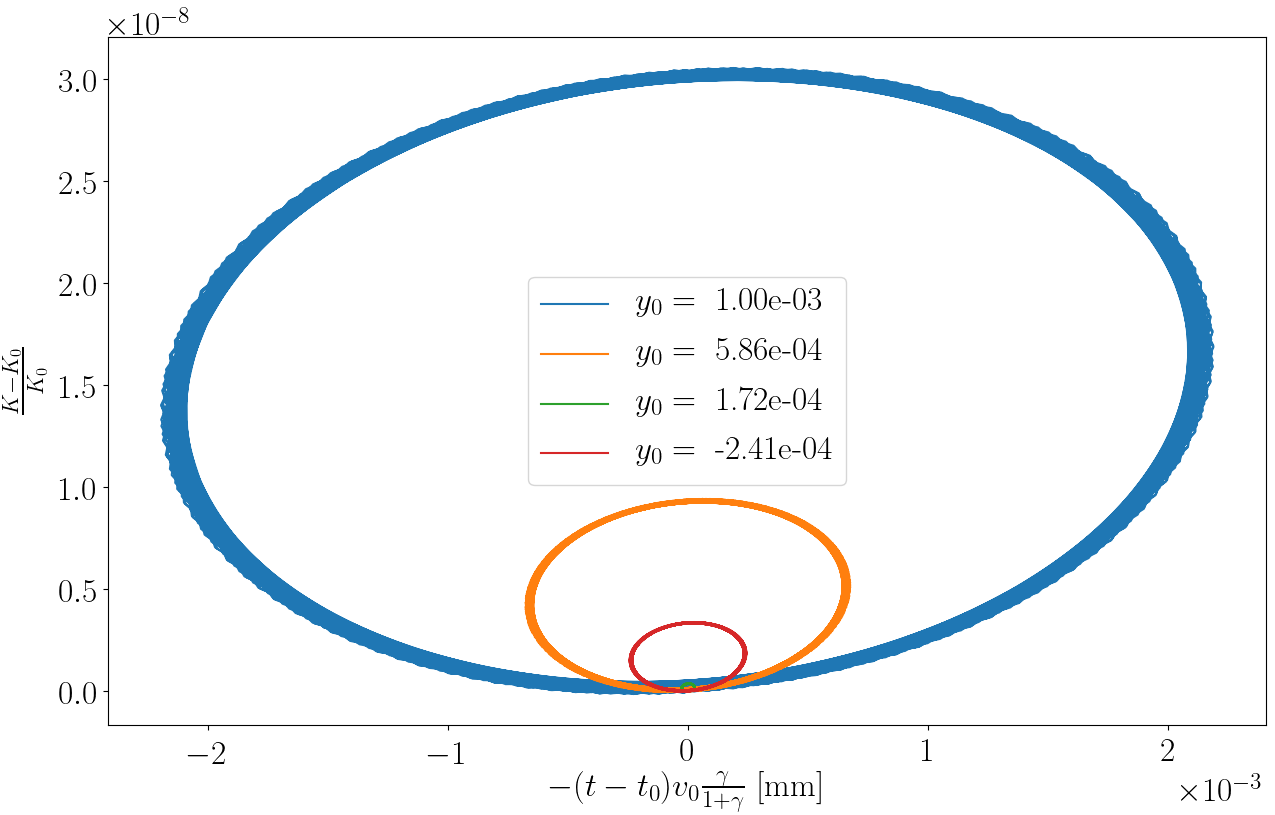
\includegraphics[height=.35\paperheight]{images/chapter1/psp_diagram_betatron}}
	\caption{Продольные фазовые портреты частиц в структуре с ВЧ продольной фокусировкой. Цветом различаются частицы с разными начальными сдвигами в вертикальной плоскости относительно референсной частицы; остальные координаты идентичны.}
\end{figure}

Мы называем равновесный уровень энергии, ассоциированный со сдвигом импульса~\eqref{eq:EquLevMom_shift},
\emph{эффективным Лоренц-фактором}:
\begin{equation}\label{eq:EffectiveGamma}
\g*= \gamma_0 + \beta_0^2\gamma_0\cdot\Delta\delta_{eq},
\end{equation}
где $\gamma_0$, $\beta_0$ Лоренц-фактор и нормализованная скорость референсной частицы.

Отметим, что понятие эффективного Лоренц-фактора позволяет нам учитывать вариацию величины спин-тюна,
вызванную вариацией длины орбиты частицы. Оно является краеугольным камнем в анализе 
декогеренции спина (рассматривается в разделе~\ref{chpt3:decoherence}) и её подавления посредством секступольных полей.

Оно также играет важную роль в успешном воспроизведении МДМ-компоненты совокупной угловой скорости
спин-прецессии.

\section{Варианты магнитооптических струкутур накопительных колец с ``замороженным,'' и ``квази-замороженным'' спином} \label{chpt1:Lattices}


Существуют два подхода к проблеме построения накопительного кольца для измерения ЭДМ дейтрона: 
\begin{enumerate*}[\itshape a\upshape)]
	\item структура с ``замороженным'' спином (FS), и 
	\item структура с ``квази-замороженным'' спином (QFS).
\end{enumerate*}

В следующих разделах мы рассмотрим возможные варианты колец обоих типов.

\section{Структура с ``замороженным'' спином} \label{sec:FS_BNL_lattice}
В структуре FS-типа, горизонтальная проекция вектора спина частицы пучка \emph{непрерывно} сонаправлена с вектором её импульса. Для реализации условия непрерывности, в такой структуре используются цилиндрические спин-ротаторы, создающие одновременно и электростатическое, и магнитное поля. На Рисунке~\ref{fig:BNL_lattice} представлен вариант кольца FS-типа.~\cite{Senichev:Lattices} Данное кольцо имеет длину 145.85 м, и рассчитано на инжекцию пучка дейтронов на энергии 270 МэВ. В структуре предусмотрено использование ВЧ-резонатора для подавления линейного эффекта декогеренции спина путём усреднения энергии вокруг значения равновесной энергии частицы. Продольное напряжение резонатора $V = 100$ кВ, частота поля $f_{RF} = 5\cdot f_{rev}$, где $f_{rev} = 1.00$ МГц --- частота оборота пучка. Остающиеся нелинейные эффекты декогеренции подавляются с помощью \hl{трёх}\footnote{У Еремея два.} семейств секступолей.

\begin{figure}[h!]
	\centering
	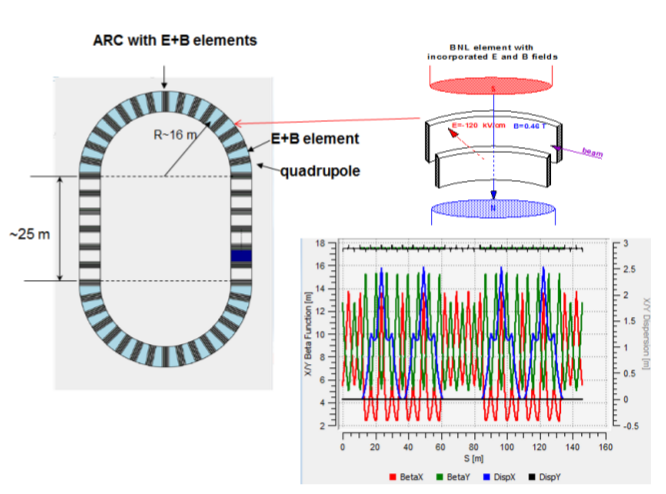
\includegraphics[width=\linewidth]{images/chapter2/BNL_lattice}
	\caption{Вариант кольца, построенного по принципу ``замороженного'' спина. В арках использованы цилиндрические электро-магнитные элементы (Рисунок взят из~\cite{Senichev:Lattices})\label{fig:BNL_lattice}}
\end{figure}

Основная цель FS-концепции кольца --- максимизация ЭДМ сигнала. Однако, следует обратить внимание на то, что строгое выполнение условия замороженности спина возможно только для референсной частицы. Это связано с тем, что, как следует из уравнения~\eqref{eq:TBMT_MDM}, для заданных E-, B-полей, существует уникальное значение Лоренц-фактора $\gamma$, при котором $\W_y^{MDM} = 0$. Таким образом, даже в FS-структуре, спин-векторы большинства частиц ``заморожены'' лишь приблизительно.

\section{Структура с ``квази-замороженным'' спином} \label{sec:QFS_concept}
В QFS-концепции кольца отказываются от непрерывного выполнения условия сонаправленности векторов поляризации и импульса пучка, требуя лишь равенства нулю \emph{совокупного за оборот} угла поворота вектора поляризации относительно импульса в электростатических ($\Phi_s^E$) и магнитных ($\Phi_s^B$) элементах:~\cite{Senichev:Lattices}
\begin{equation*}
	\sum_i \Phi_{s,i}^E = -\sum_j \Phi_{s,j}^B.
\end{equation*}

Как следует из определения спин-тюна (см. раздел~\ref{sec:TBMT_introduction}), угол поворота спин-вектора частицы относительно её импульса в электромагнитном поле $\Phi_s = \nu_s \cdot \Phi$, где $\Phi$ угол поворота импульса, а $\nu_s$ спин-тюн.

Угловая скорость поворота вектора импульса частицы в магнитном поле $\vec B$ есть 
\[
\w_B = \frac qm \frac B \gamma,
\]
в электростатическом $\vec E$:
\[
\w_E = \frac qE \frac{\vec E\times \vec\beta}{c\beta^2\gamma},
\]

из чего следуют выражения для спин-тюна частицы в электростатическом и магнитном полях:
\begin{equation}
	\begin{cases}
		\nu_s^B &= \gamma G, \\
		\nu_s^E &= \beta^2\gamma\bkt{\frac{1}{\gamma^2-1} - G}.
	\end{cases}
\end{equation}

Преимущество кольца QFS-типа над кольцом FS-типа в относительной простоте исполнения: нет необходимости использовать совмещённые цилиндрические электро-магнитные элементы; в двух вариантах QFS-кольца, рассматриваемых ниже, используются 
\begin{enumerate*}[\itshape a\upshape)]
\item либо прямые фильтры Вина, 
\item либо цилиндрические электростатические дефлекторы и магнитные диполи раздельно.
\end{enumerate*}
С другой стороны, из-за появления вертикальной компоненты оси прецессии спина $\bar n_y$, максимальная амплитуда ЭДМ-сигнала уменьшается по сравнению с полностью замороженным случаем. Фактор, на который уменьшается амплитуда~\cite{Senichev:QFS_IPAC15}
\[
J_0(\Phi_s) \approx 1 - \frac{\Phi_s^2}{4},
\]
где $\Phi_s$ есть максимальный угол отклонения горизонтальной проекции вектора спина частицы от вектора импульса. Педположим, что этот угол не превосходит половины \hl{набега спиновой фазы за оборот} $\pi\cdot \gamma G/2n$; в данном контексте $n$ --- периодичность оптики кольца. Поскольку магнитная аномалия дейтрона $G = -0.142$, для рассматриваемых ниже QFS структур $J_0\ge 0.98$.

\subsection{Структура с кодовым названием 6.3}\label{sec:QFS_6_3_lattice}

На Рисунке~\ref{fig:QFS_6_3_lattice} представлена структура, построенная по принципу квази-замороженного спина, в которой электростатические и магнитные поля разделены в пространстве.~\cite{Senichev:Lattices} Электростатические цилиндрические дефлекторы с отрицательной кривизной орбиты используются для компенсации набега фазы, связанного с МДМ-прецессией в магнитных арках.~\cite{Senichev:QFS_IPAC15} Кольцо длины 166.67 м рассчитано на инжекцию пучка дейтронов на энергии 270 МэВ. Для подавления эффектов декогеренции первого порядка используется ВЧ резонатор, с продольным полем $V = 100$ кВ, и рабочей частотой $f_{RF} = 5\cdot f_{rev}$, где $f_{rev} = 0.87$ МГц. Нелинейные эффекты декогеренции подавляются с помощью \hl{шести семейств секступолей}.

\begin{figure}[h!]
	\centering
	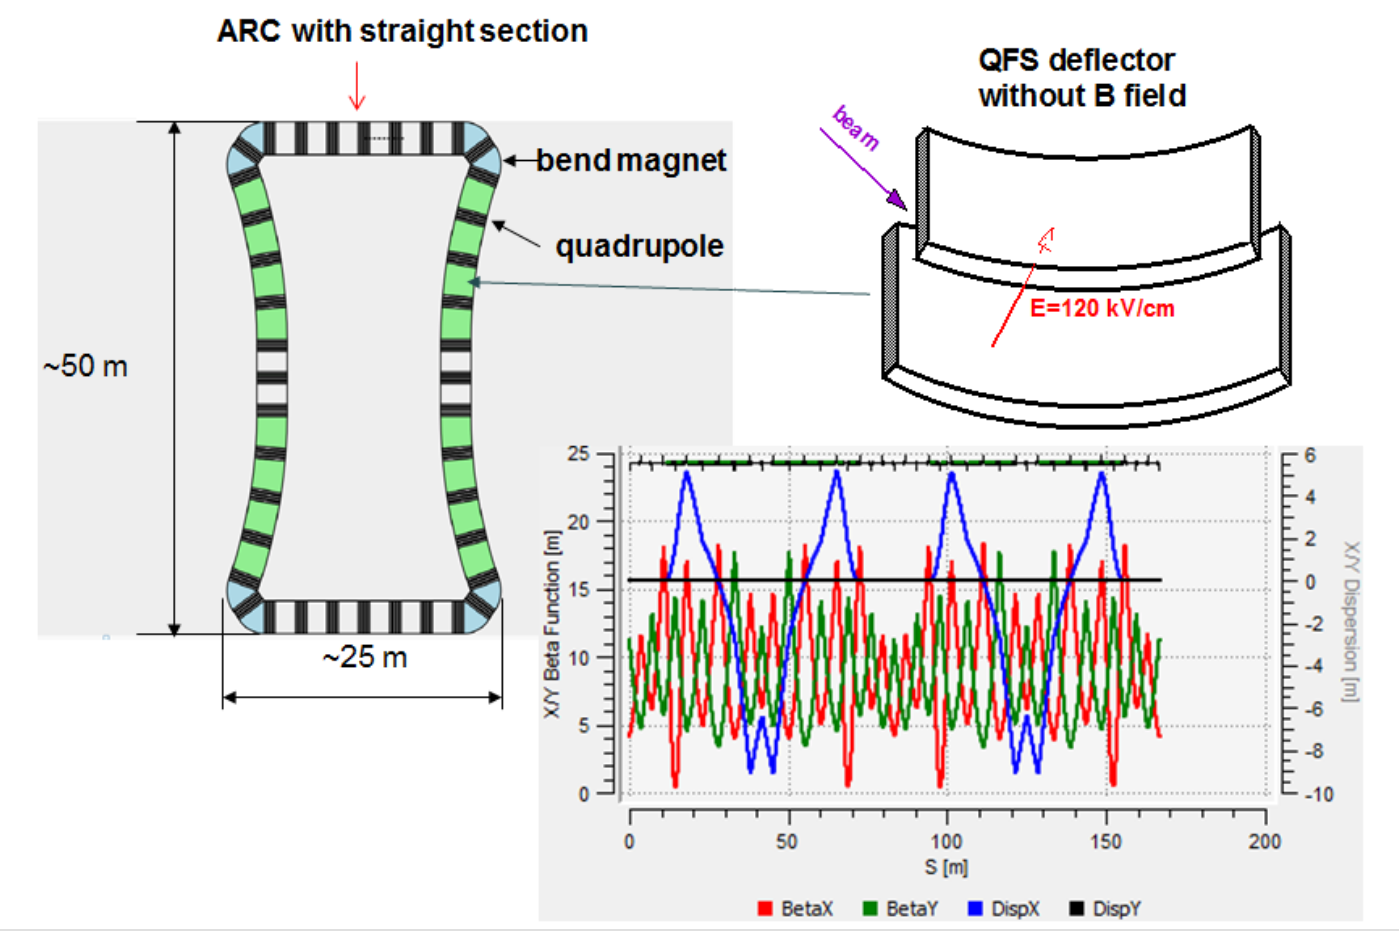
\includegraphics[width=\linewidth]{images/chapter2/6_3_lattice}
	\caption{Вариант кольца, построенного по принципу квази-замороженного спина, дизайн с разделением E- и B-полей. (Рисунок взят из~\cite{Senichev:Lattices})\label{fig:QFS_6_3_lattice}}
\end{figure}

\subsection{Структура с кодовым названием E+B}\label{sec:QFS_EB_lattice}

В структуре, представленной на Рисунке~\ref{fig:QFS_E+B_lattice}, используются прямые, статические фильтры Вина. Это позволяет:
\begin{enumerate*}[\itshape a\upshape)]
	\item исключить нелинейные компоненты электростатического поля, возникающие в связи с кривизной дефлектора, и 
	\item упростить структуру с инженерной точки зрения.
\end{enumerate*}

Длина структуры 149.21 м, энергия инжектируемых дейтронов 270 МэВ. Для подавления эффекта декогеренции первого порядка используется ВЧ-резонатор с продольным напряжением $V = 100$ кВ и частотой $f_{RF} = 5\cdot f_{rev}$, где $f_{rev} = 0.98$ МГц. Нелинейные эффекты декогеренции подавляются с помощью \hl{четырёх семейств секступолей}.
\begin{figure}[h!]
	\centering
	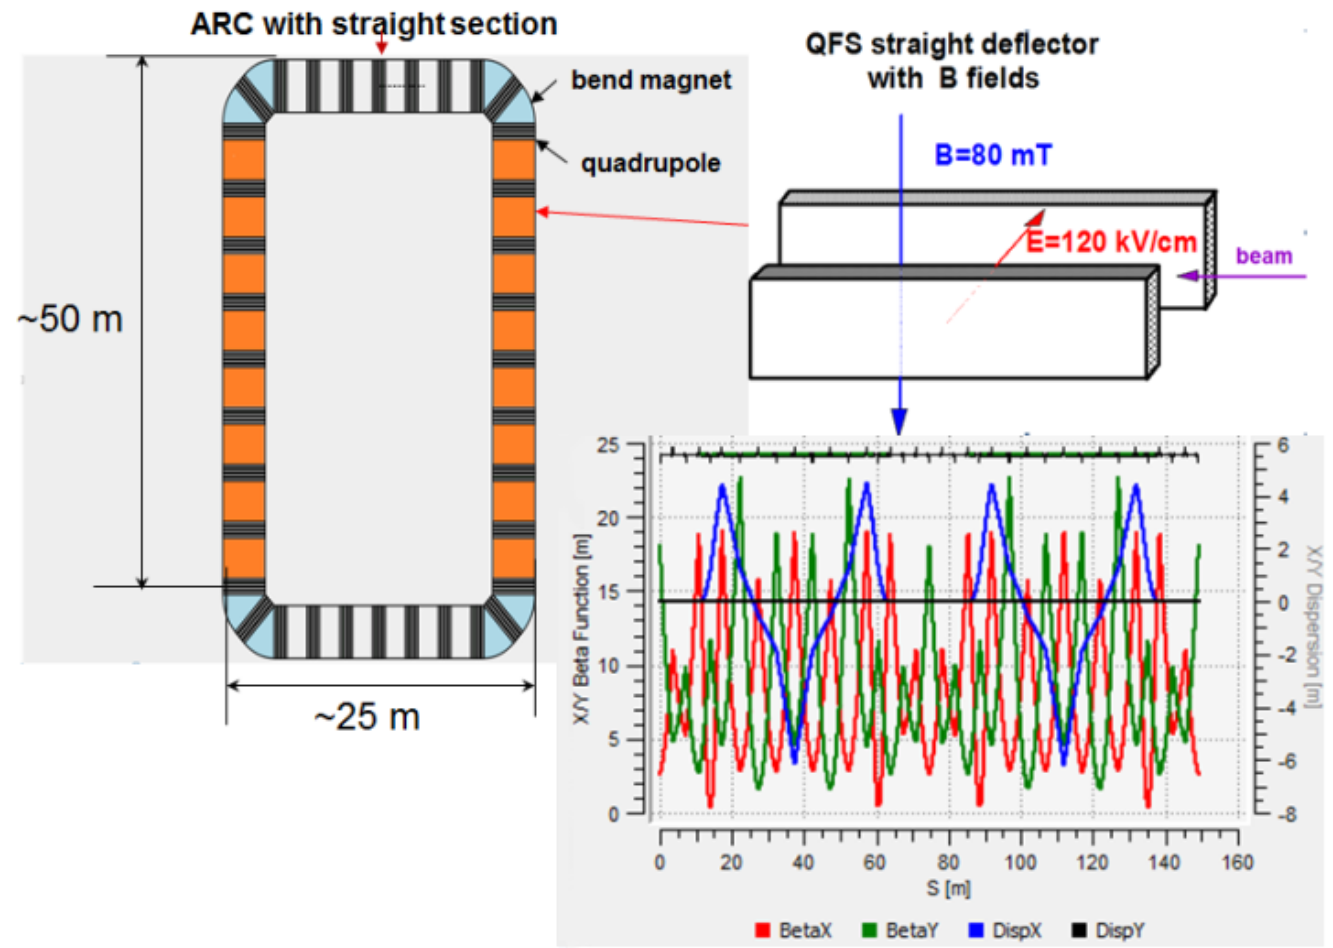
\includegraphics[width=\linewidth]{images/chapter2/E+B_lattice}
	\caption{Вариант кольца, построенного по принципу квази-замороженного спина, дизайн с прямыми фильтрами Вина. (Рисунок взят из~\cite{Senichev:Lattices})\label{fig:QFS_E+B_lattice}}
\end{figure}



\clearpage